\documentclass[a4paper]{book}

\usepackage{amsmath}
\usepackage{amssymb}
\usepackage[hypcap=false]{caption}
\usepackage{enumitem}	% 定制enumerate标号
\usepackage{geometry}
\geometry{
	left=2cm,
	right=2cm,
	top=2cm,
	bottom=2cm,
}
\usepackage{graphics}
\usepackage{hyperref}
\hypersetup{
    colorlinks=true,            %链接颜色
    linkcolor=blue,             %内部链接
    filecolor=magenta,          %本地文档
    urlcolor=cyan,              %网址链接
}
\usepackage[none]{hyphenat}		% 阻止长单词分在两行
\usepackage{mathrsfs}
\usepackage[version=4]{mhchem}
\usepackage{subcaption}
\usepackage{titlesec}

\RequirePackage[many]{tcolorbox}
\tcbset{
    boxed title style={colback=magenta},
	breakable,
	enhanced,
	sharp corners,
	attach boxed title to top left={yshift=-\tcboxedtitleheight,  yshifttext=-.75\baselineskip},
	boxed title style={boxsep=1pt,sharp corners},
    fonttitle=\bfseries\sffamily,
}

\definecolor{skyblue}{rgb}{0.54, 0.81, 0.94}

\newtcolorbox[auto counter, number within=chapter, number format=\arabic]{exercise}[1][]{
    title={Exercise~\thetcbcounter},
    colframe=skyblue,
    colback=skyblue!12!white,
    boxed title style={colback=skyblue},
    overlay unbroken and first={
        \node[below right,font=\small,color=skyblue,text width=.8\linewidth]
        at (title.north east) {#1};
    }
}

\newtcolorbox[auto counter, number within=chapter, number format=\arabic]{solution}[1][]{
    title={Solution~\thetcbcounter},
    colframe=teal!60!green,
    colback=green!12!white,
    boxed title style={colback=teal!60!green},
    overlay unbroken and first={
        \node[below right,font=\small,color=red,text width=.8\linewidth]
        at (title.north east) {#1};
    }
}

% special new commands for common symbols used in the article
\newcommand\la{\langle}
\newcommand\ra{\rangle}
\newcommand\lr[2]{\langle#1\|#2\rangle}
\newcommand\tr[1]{\mathrm{tr(#1)}}
\newcommand\Tr[3]{#1\mathrm\#2#3}
\newcommand*{\dif}{\mathop{}\!\mathrm{d}}
\renewcommand\det[1]{\mathrm{det\left(#1\right)}}
\newcommand{\HF}{{\rm HF}}

\newcommand{\A}{{\bf A}}
\newcommand{\B}{{\bf B}}
\newcommand{\C}{{\bf C}}
\newcommand{\I}{{\bf 1}}
\newcommand{\U}{{\bf U}}
\newcommand{\Op}{{\bf O}}

\titleformat{\chapter}[display]
  {\bfseries\Large}
  {\filright\MakeUppercase{\chaptertitlename} \Huge\thechapter}
  {1ex}
  {\titlerule\vspace{1ex}\filleft}
  [\vspace{1ex}\titlerule]
  
\allowdisplaybreaks

\begin{document}

	\stepcounter{chapter}\stepcounter{chapter}\stepcounter{chapter}\stepcounter{chapter}\stepcounter{chapter}

	\chapter{Many-Body Perturbation Theory}
	
	\section{Rayleigh-Schr{\"o}dinger (RS) Perturbation Theory}
	
	\section{Diagrammatic Representation of RS Perturbation Theory}
	
	\subsection{Diagrammatic Perturbation Theory for Two States}
	
	\begin{exercise}
	Write down and evaluate all fifth-order diagrams that have the property that an imaginary horizontal line crosses only one hole and one particle line. Show that the sum of such diagrams is
	\[
		\frac{V_{12}V_{21}(V_{22}-V_{11})^3}{(E^{(0)}_1 - E^{(0)}_2)^4}
	\]
	{\it Hint}: There are eight such diagrams, and they can be generated by adding three dots to the second-order diagram in all positive ways.
	\end{exercise}
	
	\begin{solution}
		6-1 so
	\end{solution}
	
	\subsection{Diagrammatic Perturbation Theory for \texorpdfstring{$N$}- States}
	
	\begin{exercise}
	Use diagrammatic techniques to obtain the fourth-order perturbation energy of a particular state (say, $i$) of an $N$-state system. That is, evaluate the diagrams
	
	\begin{center}
	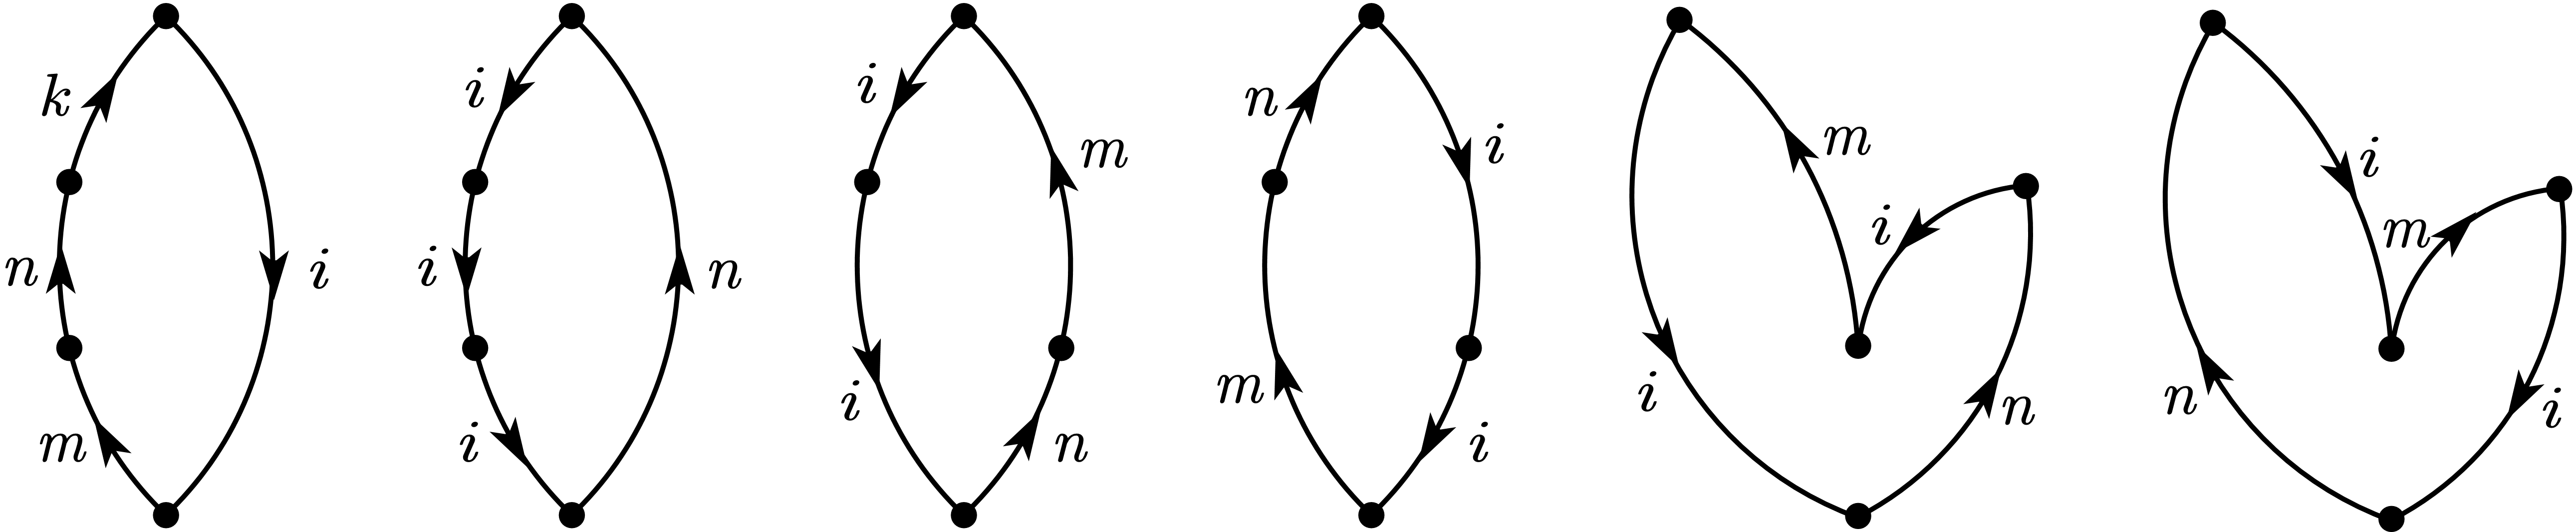
\includegraphics[scale=1.0]{./pictures/336.png}
	\captionof{figure}{1111}
	\end{center}
	
	where the indices $m$, $n$, $k$, ... exclude $i$. Using the approach of Section 6.1, obtain an algebraic expression for the fourth-order energy and compare it to the diagrammatic result.
	
	\end{exercise}
	
	\begin{solution}
		6-2 so
		
		fffff
	\end{solution}
	
	\subsection{Summation of Diagrams}
	
	\section{Orbital Perturbation Theory: One-Particle Perturbations}
	
	\begin{exercise}
	Derive
	\[
		E^{(2)}_0 = \sum_{ar} \frac{v_{ar}v_{ra}}{\varepsilon^{(0)}_a - \varepsilon^{(0)}_r}
	\]
	starting with the general expression for the second-order energy (Eq.(6.12)) applied to an $N$-electron system,
	\[
		E^{(2)}_0 = \sum_n {}^\prime \frac{\left| \langle \Psi_0 | \displaystyle\sum_i v(i)| n \rangle \right|^2 }{E^{(0)}_0-E^{(0)}_n}
	\]
	where the sum runs over all states of the system except the ground state.
	
	{\it Hint}: The states $| n \rangle$ must be single excitations of the type
	\[
		|\Psi^r_a\rangle = | \chi^{(0)}_1 \cdots \chi^{(0)}_{a-1} \chi^{(0)}_{r} \chi^{(0)}_{a+1} \cdots \chi^{(0)}_{N} \rangle.
	\]
	\end{exercise}
	
	\begin{solution}
		6-3 so
	\end{solution}
	
	\begin{exercise}
	Calculate the third-order energy $E^{(3)}_0$ using the general expression given in Eq.(6.15).
	\begin{enumerate}
	
	\item[a.] Show that
	\[
		B^{(3)}_0 = - E^{(1)}_0 \sum_n {}^\prime \frac{|\langle \Psi_0 | \mathscr{V} | n \rangle |^2}{(E^{(0)}_0-E^{(0)}_n)^2} = - \sum_{abr} \frac{v_{aa} v_{rb} v_{br}}{( \varepsilon^{(0)}_b - \varepsilon^{(0)}_r)^2}.
	\]
		
	\item[b.] Show that
	\[
		A^{(3)}_0 = \sum_{nm} {}^\prime \frac{\langle \Psi_0 | \mathscr{V} | n \rangle \langle n | \mathscr{V} | m \rangle \langle m | \mathscr{V} | \Psi_0 \rangle}{(E^{(0)}_0-E^{(0)}_n)(E^{(0)}_0-E^{(0)}_m)} = \sum_{abrs} \frac{v_{ar} v_{sb} \langle \Psi^r_a | \mathscr{V} | \Psi^s_b \rangle}{( \varepsilon^{(0)}_a - \varepsilon^{(0)}_r)( \varepsilon^{(0)}_b - \varepsilon^{(0)}_s)}.
	\]
	
	\item[c.] Show that
	\begin{align*}
		\langle \Psi^r_a | \mathscr{V} | \Psi^s_b \rangle &= v_{rs} & \text{if} \, a = b  \quad r \neq s, \\
		&= - v_{ba} & \text{if} \, a \neq b \quad r = s, \\
		&= \sum_{c} v_{cc} - v_{aa} + v_{rr} & \text{if} \, a = b \quad r = s , \\
		&= 0 & \text{otherwise}.
	\end{align*}
		
	\item[d.] Finally, combine the two terms to obtain
	\[
		E^{(3)}_0 = A^{(3)}_0 + B^{(3)}_0 = \sum_{ars} \frac{v_{ar} v_{rs} v_{sa}}{( \varepsilon^{(0)}_a - \varepsilon^{(0)}_r)( \varepsilon^{(0)}_a - \varepsilon^{(0)}_s)} - \sum_{abr} \frac{v_{ra} v_{ab} v_{br}}{( \varepsilon^{(0)}_a - \varepsilon^{(0)}_r) ( \varepsilon^{(0)}_b - \varepsilon^{(0)}_r)}.
	\]
	
	\item[e.] Show that for a chosed-shell system
	\[
		E^{(3)}_0 = 2\sum_{ars}^{N/2} \frac{v_{ar} v_{rs} v_{sa}}{( \varepsilon^{(0)}_a - \varepsilon^{(0)}_r)( \varepsilon^{(0)}_a - \varepsilon^{(0)}_s)} - 2\sum_{abr}^{N/2} \frac{v_{ra} v_{ab} v_{br}}{( \varepsilon^{(0)}_a - \varepsilon^{(0)}_r) ( \varepsilon^{(0)}_b - \varepsilon^{(0)}_r)}.
	\]
	
	\end{enumerate}
	\end{exercise}
	
	\begin{solution}
		6-4 so
	\end{solution}
	
	\begin{exercise}
	Show that the second term in Eq.(6.52) is equal to $\frac{3}{8}\beta$ for benzene.
	\end{exercise}
	
	\begin{solution}
		6-5 so
	\end{solution}
	
	\begin{exercise}
	Consider a cyclic polyene with $N = 4\nu+2$, $\nu=1$, $2$, ... carbons. Instead of assuming that all the bonds are identical, suppose they alternate in length. In the context of H{\"u}ckel theory this means that the resonance integrals between adjacent carbons are not all equal to $\beta$ but alternate between $\beta_11$ and $\beta_2$. For example, for benzene we have
	
	\begin{center}
	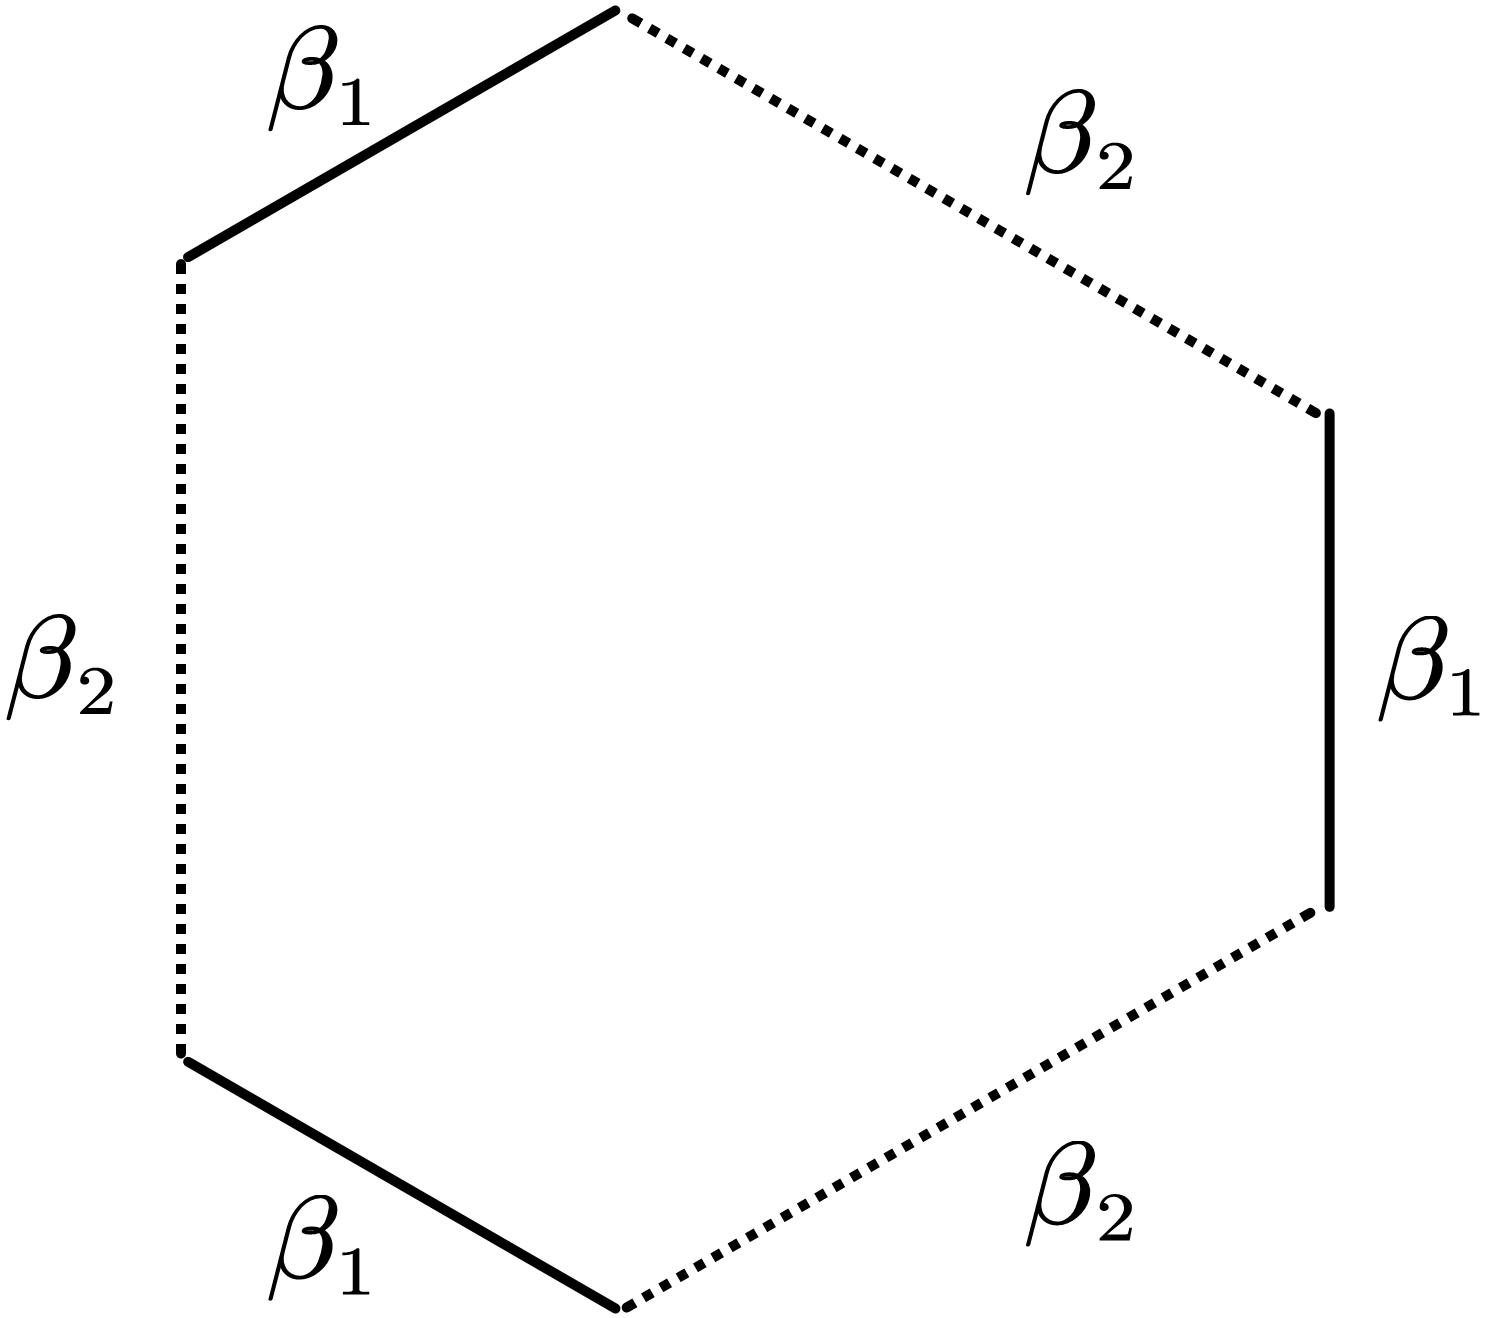
\includegraphics[scale=1.2]{./pictures/346.png}
	\captionof{figure}{1111}
	\end{center}
	
	Now it can be shown that the exact energy for a cyclic polyene of this type is
	\[
		\mathscr{E}_0 = N \alpha - 2 \sum_{j=-\nu}^\nu \left( \beta^2_1 + \beta^2_2 + 2 \beta_1 \beta_2 \cos{\frac{2j\pi}{2\nu+1}} \right)^{1/2}
	\]
	(see for example, L. Salem, {\it Molecular Orbital Theory of Conjugated Systems}, Benjamin, New York, 1966, pp.498-500). Note that when $\beta_1 = \beta_2 = \beta$, since $2\cos^2\theta=(1+\cos2\theta)$ and $\beta$ is negative, we recover
	\[
		\mathscr{E}_0 = N \alpha + 4 \beta \sum_{j=-\nu}^\nu \cos{\frac{j\pi}{2\nu+1}}
	\]
	which is the result quoted in Subsection 5.3.2. Also note that when $\beta_1=\beta$ but $\beta_2=0$, we have
	\[
		\mathscr{E}_0 = N \alpha + N \beta
	\]
	which is just the total energy of the polyene using the localized ethylenic description. The purpose of this exercise is to obtain the perturbation expansion for the resonance energy by expanding the exact energy in powers of $\beta_2/\beta_1$.
	\begin{enumerate}
	
	\item[a.] Show that for benzene ($\nu=1$) the exact ground state energy in the alternating short and long bond model is
	\[
		\mathscr{E}_0 = 6 \alpha + 2(\beta_1 + \beta_2) - 4 ( \beta^2_1 + \beta^2_2 - \beta_1 \beta_2 )^{1/2}
	\]
	Do this first by using the general expression and then by setting up the H{\"u}ckel matrix, diagonalizing it and adding up the occupied orbital energies. Note that when $\beta_1=\beta_2=\beta$ we recover our old result, $6\alpha+8\beta$.
	
	\item[b.] Setting $\beta_1 = \beta$ and $\beta_2/\beta_1=x$ show that the resonance energy of benzene can be written as
	\[
		E_R = 4 \beta ( \frac{1}{2}x - 1 + (1-x+x^2)^{1/2})
	\]
	Note that when $x=0$, $E_R=0$ and when $x=1$, $E_R=2\beta$ which is exact.
	
	\item[c.] Using the relation
	\[
		(1 + y)^{1/2} = 1 + \frac{1}{2} y - \frac{1}{8}y^2 + \frac{1}{16} y^3 - \frac{5}{128}y^4 + \cdots , \quad |y|<1
	\]	
	expand $E_R$ to fourth order in x and thus show that
	\[
		E_R = \beta ( \frac{3}{2}x^2 + \frac{3}{4} x^3 + \frac{3}{32}x^4 + \cdots )
	\]
	Identifying the coefficient of $x^n$ with the $n$th-order perturbation result (i.e., $E^(n)_0$), we have
	\begin{align*}
		E^{(2)}_0 &= \frac{3}{2} \beta, \\
		E^{(3)}_0 &= \frac{3}{4} \beta, \\
		E^{(4)}_0 &= \frac{3}{32} \beta.
	\end{align*}
	Note that $E^{(2)}_0$ and $E^{(3)}_0$ agree with our previously calculated values. This derivation provides some insight into the poor convergence of the perturbation expansion of the resonance energy of benzene. Basically, the perturbation expansion converges rapidly when $x$ is small. However, for our problem $x$ is equal to unity.
	
	The resonance energy calculated up to $M$th-order as a function of $M$ is shown below. Note the oscillatory convergence towards the exact value to $2\beta$. The method used above to obtain $E^{(n)}_0$ for $n=2,3,4$ becomes extremely laborious for larger $n$. The results below were calculated by first showing that $E^{(n)}_0 = 4\beta C^{-1/2}_n(1/2)$, where $C^{-1/2}_n(x)$ is a Gegenbauer polynomial of degree $n$ and order $-\frac{1}{2}$, and then using the recursive properties of these polynomials, to show that
	\[
		(n+1)E^{(n+1)}_0 = (n-1) E^{(n)}_0 - (n-2) E^{(n-1)}_0.
	\]
	
	\begin{center}
	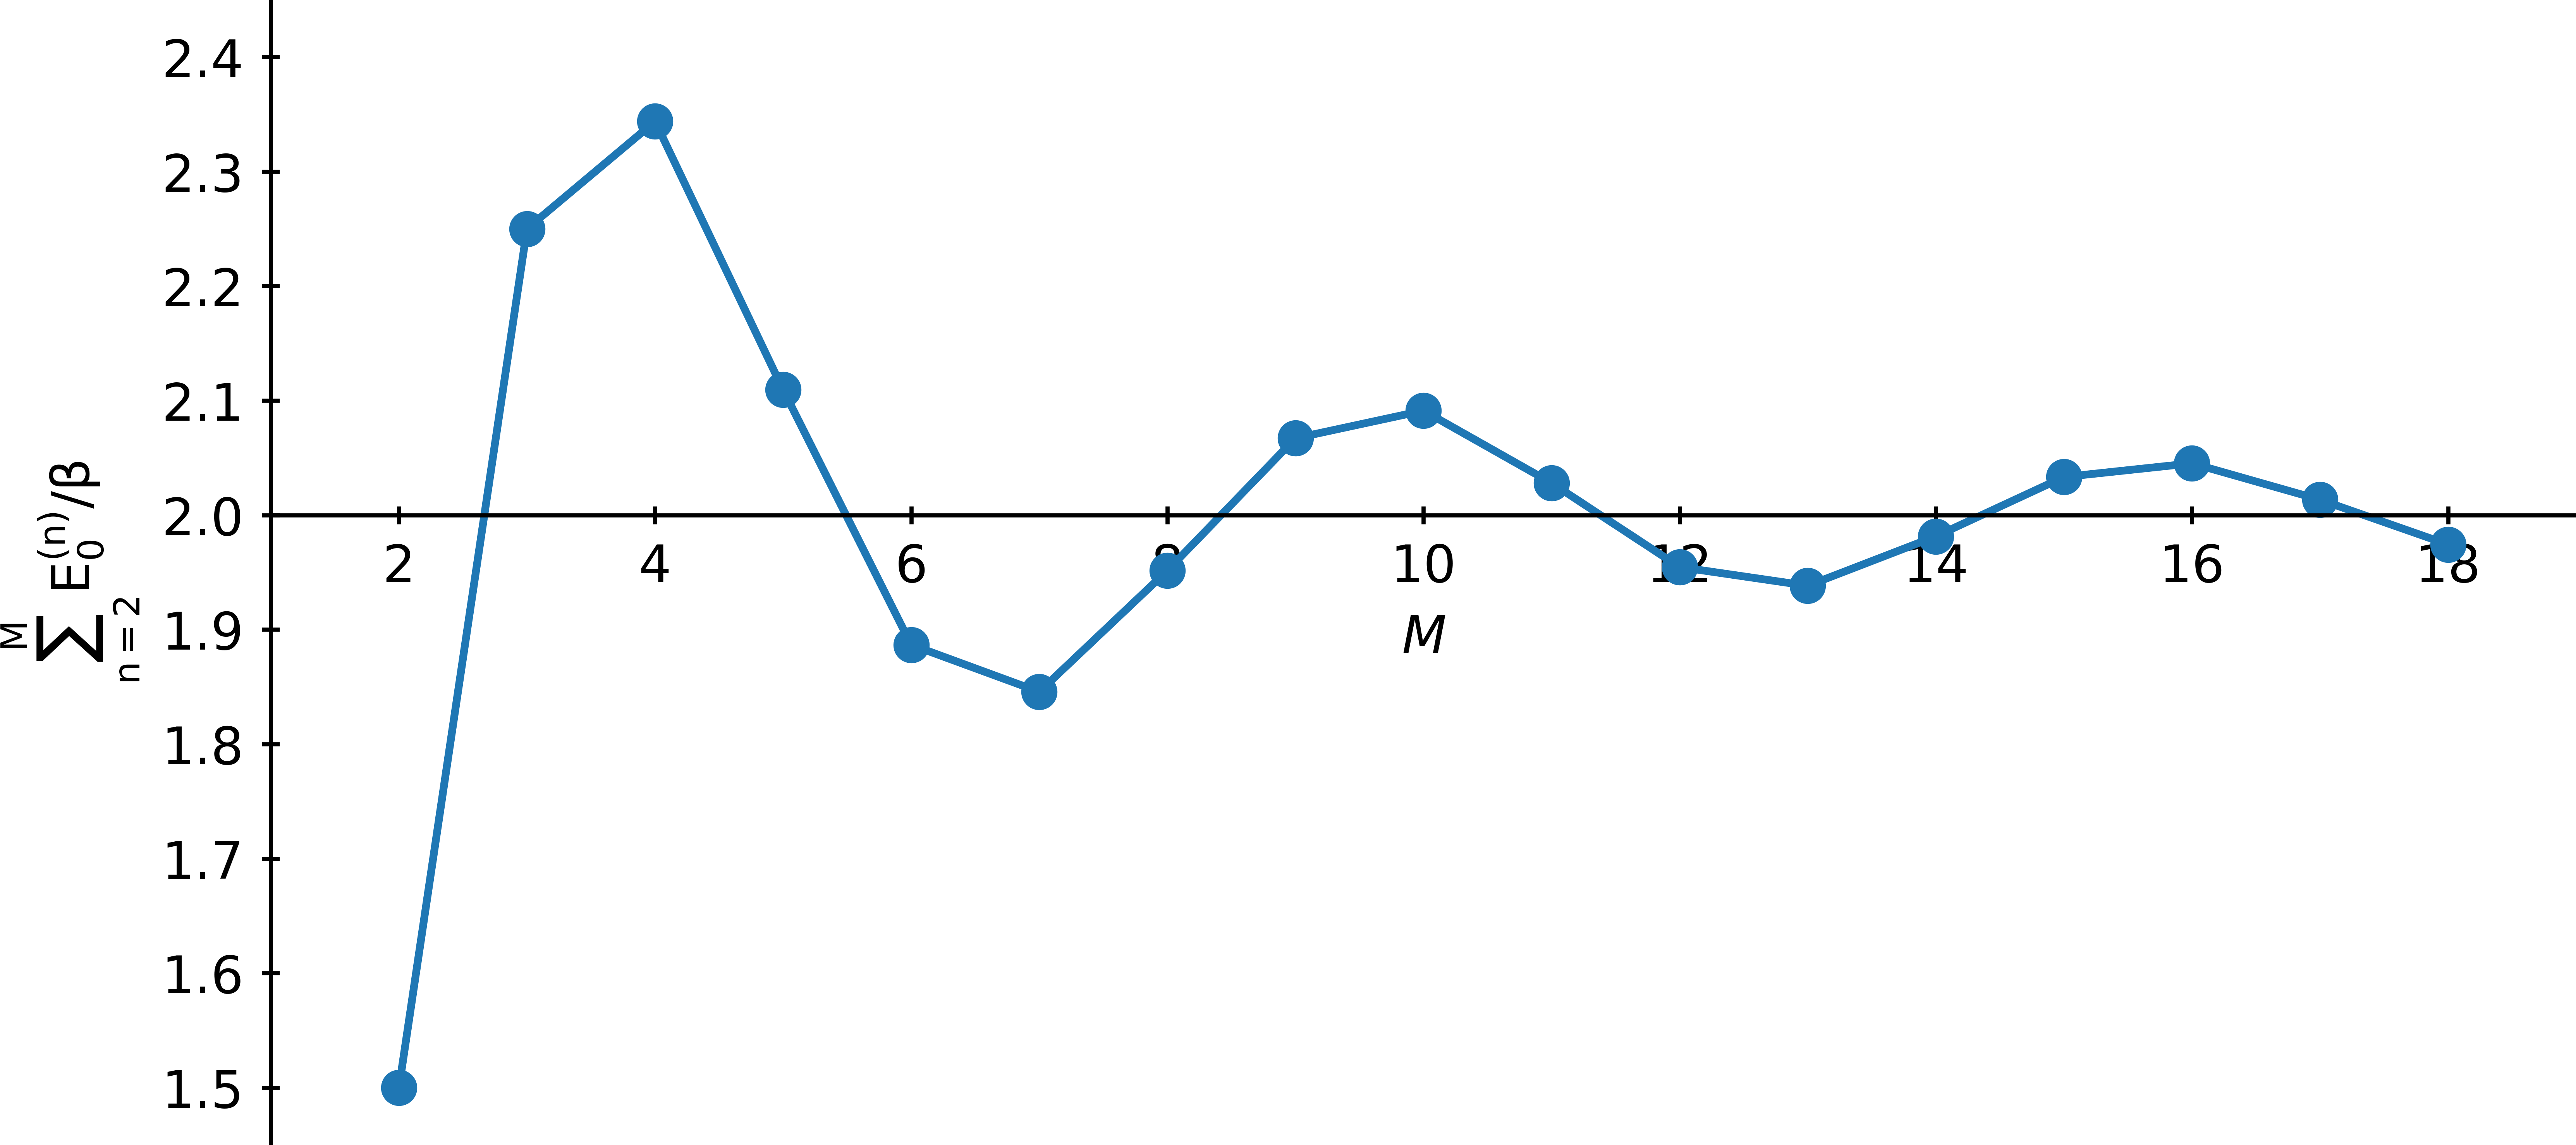
\includegraphics[scale=0.8]{./pictures/gegenbauer.png}
	\captionof{figure}{1111}\label{fig:octahedral}	
	\end{center}
	
	\end{enumerate}
	
	\end{exercise}
	
	\begin{solution}
		6-6 so
		
		ffff
		
		ffff
		
		fffff
		
	\end{solution}
	
	\section{Diagrammatic Representation of Orbital Perturbation Theory}
	
	\begin{exercise}
	Find the fourth-order energy for a closed-shell cyclic polyene.
	\begin{enumerate}
	
	\item[a.] Show that
	
	\begin{center}
	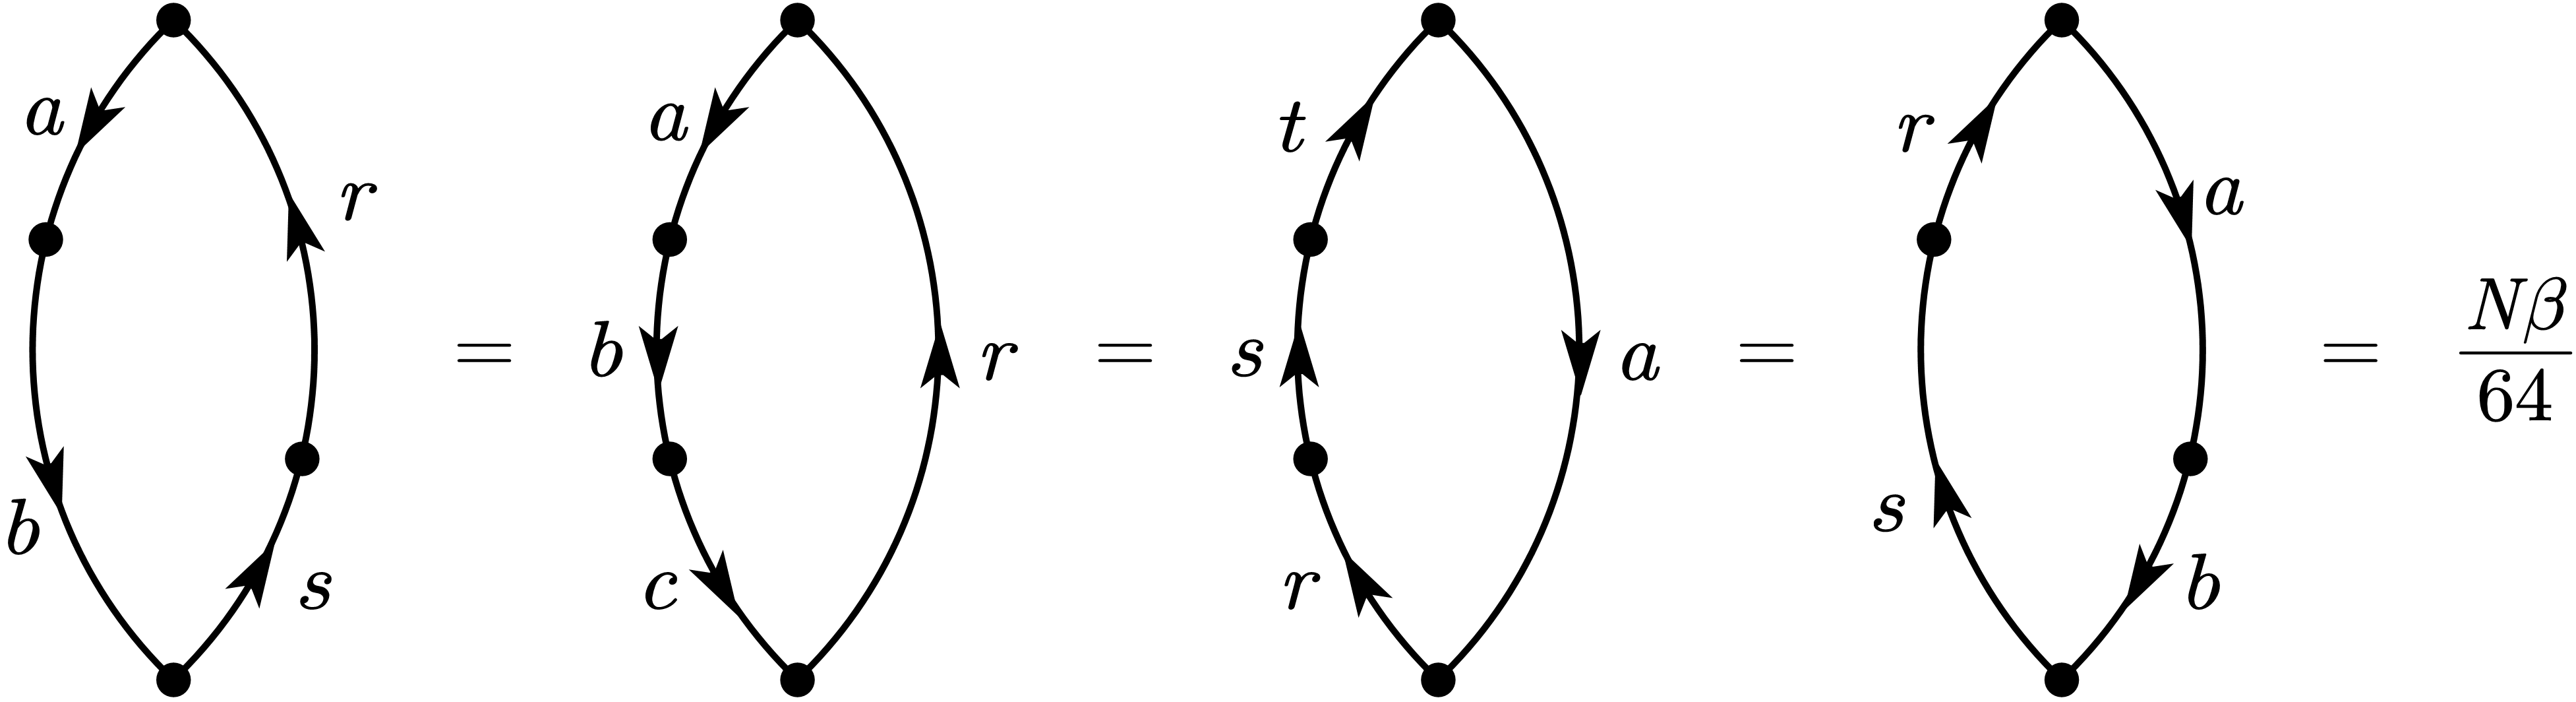
\includegraphics[scale=1.0]{./pictures/3491.png}
	\end{center}
	
	and
	
	\begin{center}
	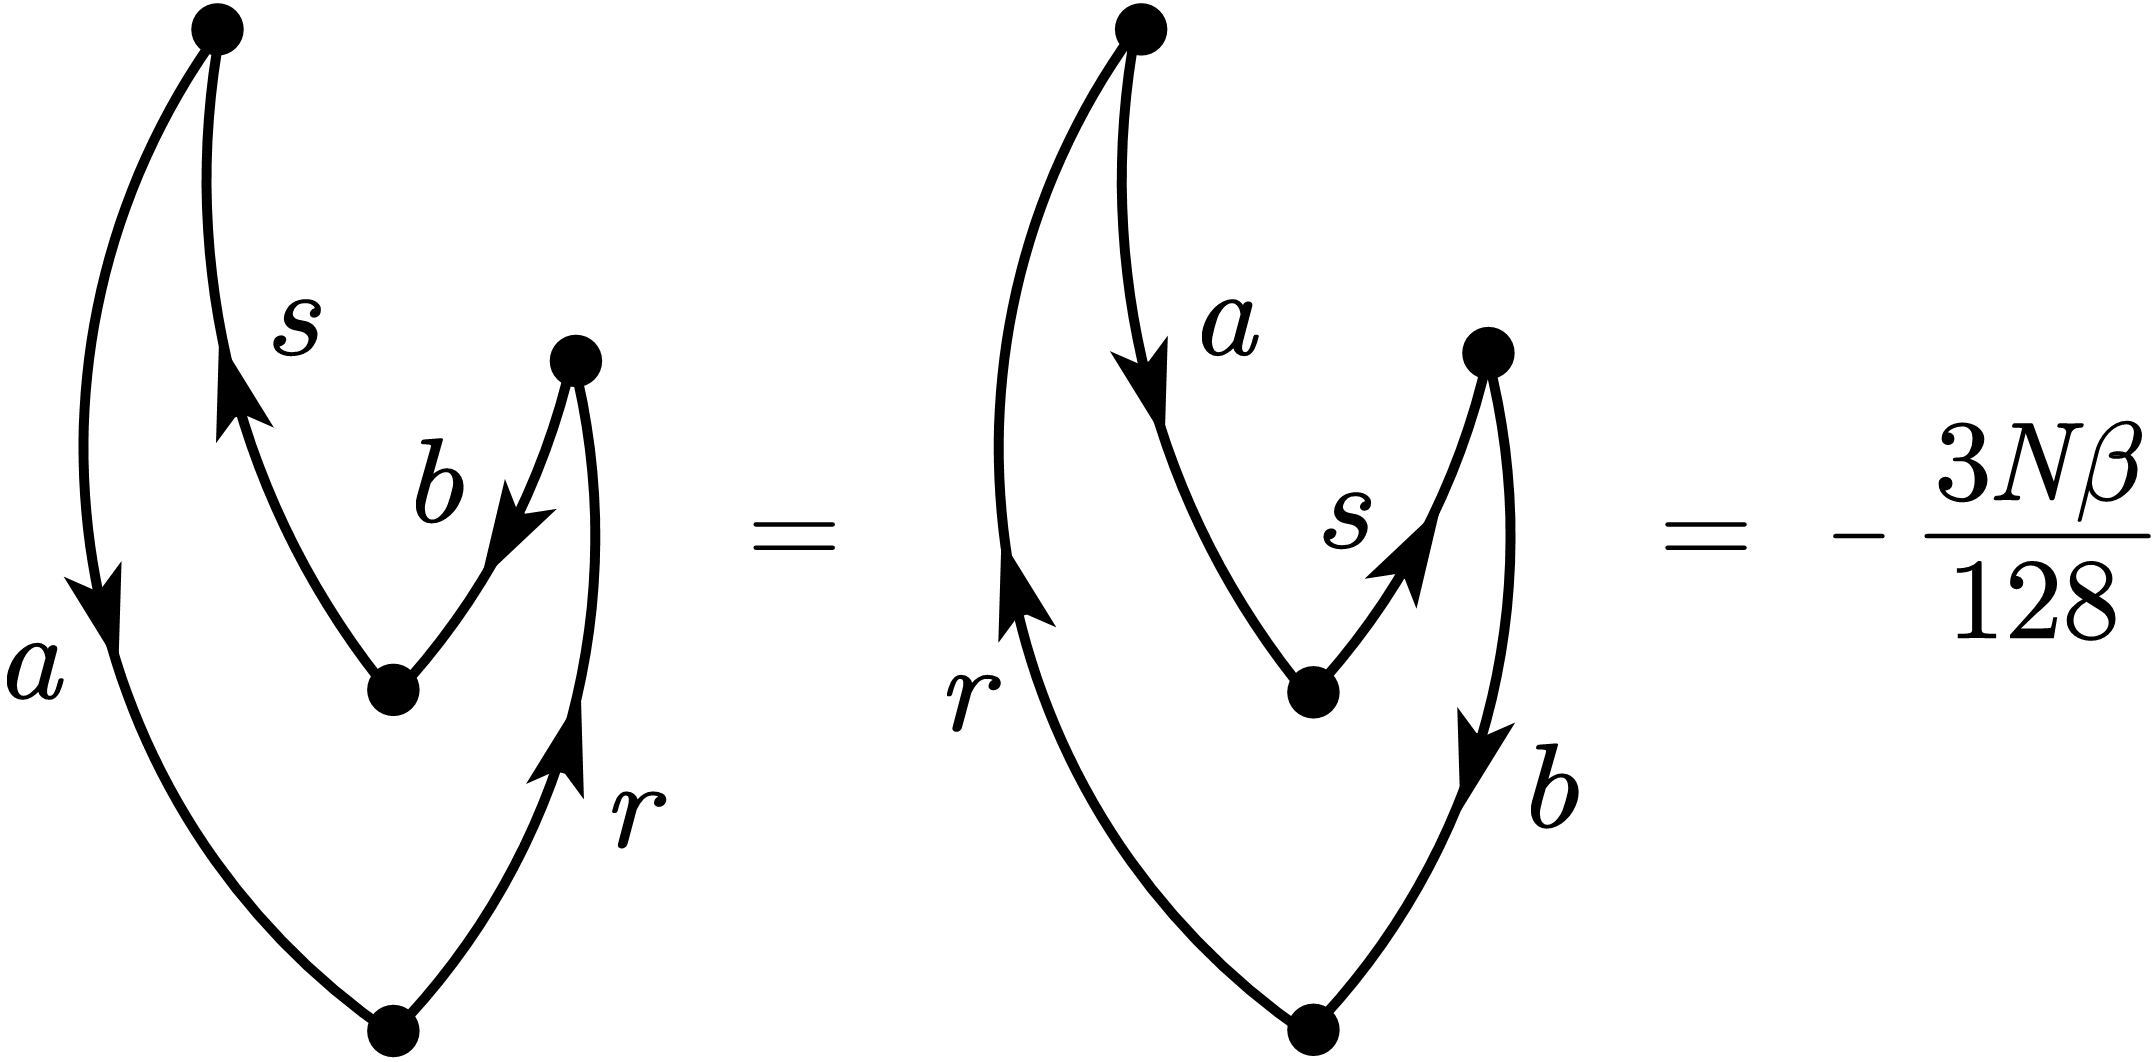
\includegraphics[scale=1.0]{./pictures/3492.png}
	\end{center}
	
	so that
	\[
		E^{(4)}_0 = \frac{N\beta}{64}
	\]
	Thus the resonance energy calculated for a cyclic polyene with $N>6$ up to fourth order is (1/4 + 1/64)$N\beta = 0.2656N\beta$, which compares very favorably with the asymptotically exact value of 0.2732$\beta$ (i.e., 97\%).
	
	\item[b.] For benzene, show that the diagrammatic result for the fourth-order energy agrees with the independently calculated result found in Exercise 6.6.
	
	\end{enumerate}		
	
	
	\end{exercise}
	
	\begin{solution}
		6-7 so
	\end{solution}
	
	\section{Perturbation Expansion of the Correlation Energy}
	
	\begin{exercise}
	Derive Eqs.(6.73) and (6.74) starting with Eq.(6.72).
	\end{exercise}
	
	\begin{solution}
		6-8 so
	\end{solution}
	
	\begin{exercise}
	Derive Eqs.(6.77) and (6.78) from Eq.(6.76).
	\end{exercise}
	
	\begin{solution}
		6-9 so
	\end{solution}
	
	\section{The \texorpdfstring{$N$}--Dependence of the RS Perturbation Expansion}
	
	\begin{exercise}
	Derive Eqs.(6.80b) and (6.90).
	\end{exercise}
	
	\begin{solution}
		6-10 so
	\end{solution}
	
	\section{Diagrammatic Representation of the Perturbation Expansion of the Correlation Energy}
	
	\subsection{Hugenholtz Diagrams}
	
	\begin{exercise}
	Show that the fourth-order diagram
	
	\begin{center}
	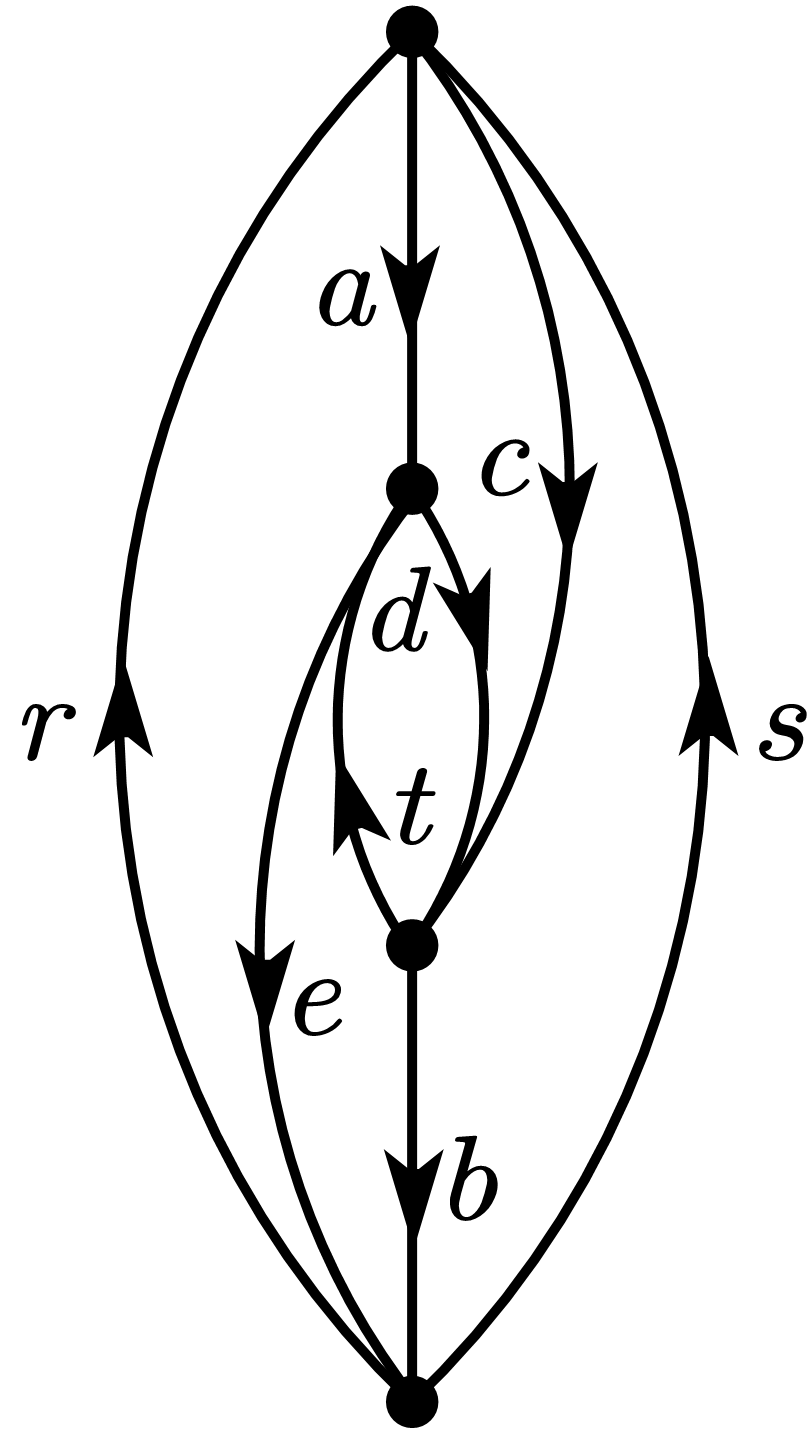
\includegraphics[scale=1.0]{./pictures/362.png}
	\end{center}
	
	is equal to
	\[
		-\frac{1}{2} \sum_{abcderst} \frac{ \lr{rs}{ac} \lr{at}{de} \lr{dc}{tb} \lr{eb}{rs} }{ ( \varepsilon_a + \varepsilon_c - \varepsilon_r - \varepsilon_s ) ( \varepsilon_c + \varepsilon_d + \varepsilon_e - \varepsilon_r - \varepsilon_t - \varepsilon_s ) ( \varepsilon_b + \varepsilon_e - \varepsilon_r - \varepsilon_s ) }.
	\]	
	
	\end{exercise}
	
	\begin{solution}
		6-11 so
	\end{solution}
	
	\subsection{Goldstone Diagrams}
	
	\begin{exercise}
	We stated that the Goldstone diagrams in Table 6.2 can be obtained by ``pulling apart" the second- and third-order Hugenholtz diagrams. This is quite tricky to see but the converse is much easier. For example, if we push
	
	\begin{center}
	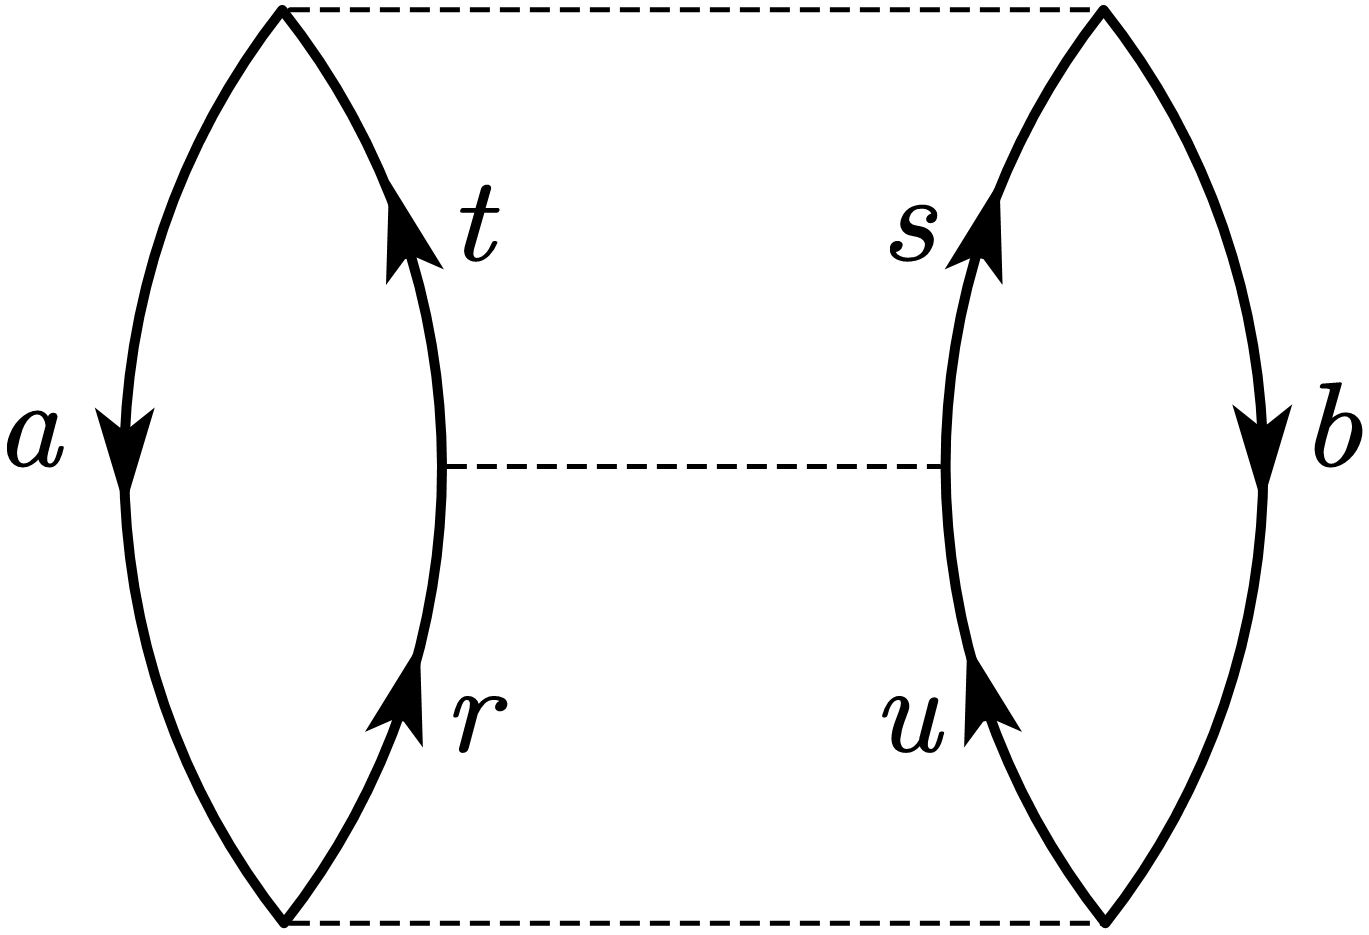
\includegraphics[scale=1.0]{./pictures/3671.png}
	\end{center}
	
	together, it is clear that we obtain
	
	\begin{center}
	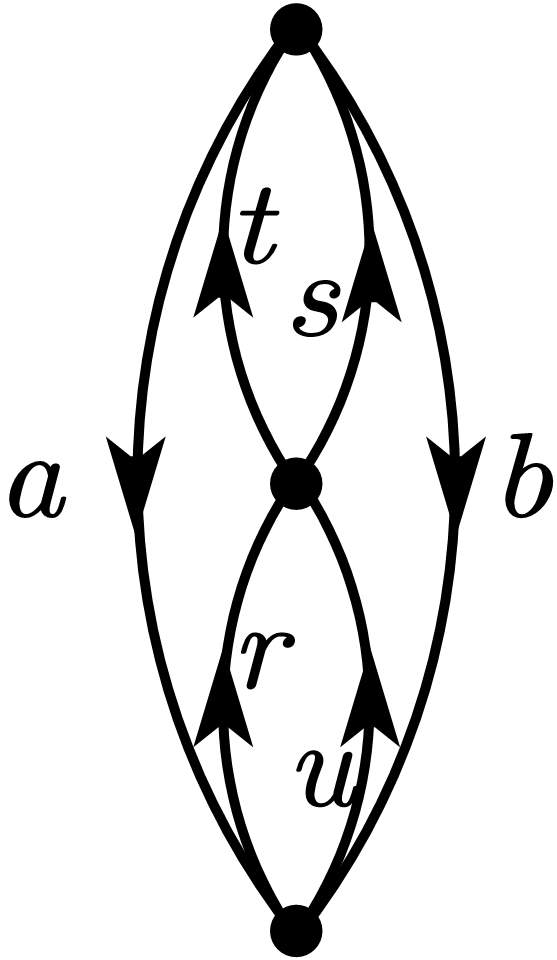
\includegraphics[scale=1.0]{./pictures/3672.png}
	\end{center}
	
	Push all third-order diagrams in Table 6.2 together in a similar way and, thus, find which Goldstone diagram comes from which Hugenholtz diagram. For the above Hugenholtz diagram, verify that its mathematical value is indeed the sum of the values of the corresponding Goldstone diagrams.
	
	\end{exercise}
	
	\begin{solution}
		6-12 so
	\end{solution}
	
	\subsection{Summation of Diagrams}
	
	\subsection{What Is the Linked Cluster Theorem?}
	
	\begin{exercise}
	Calculate $E^{(3)}_0$ for a supermolecule consisting of $N$ non-interacting minimal basis $\ce{H2}$ molecules by evaluating the Goldstone diagrams in Table 6.2. Compare your result with that of Eq.(6.92), which was obtained algebraically by explicitly cancelling terms proportional to $N^2$.
	
	{\it Hint}: Simply show that the value of each Goldstone diagram for the supermolecule in $N$ times the result for a single molecule.
	\end{exercise}
	
	\begin{solution}
		6-13 so
	\end{solution}
	
	\section{Some Illustrative Calculations}


\end{document}
